\subsubsection{Parser: Parse LLVM IR to Module Instruction}

\begin{itemize}
    \item IR Module

IR is composed of the following multi level structures:
\begin{lstlisting}[language={}]
module -> function -> value -> types
\end{lstlisting}

(1) Module structure contains Target which contains triple and datalayout information, Function, Attribute and GlobalVariable.

(2) Function structure contains Name, Type information, Visibility, Attribute and Parameter list basic information and DataLayout.

(3) Datalayout contains the sequential logical relationship between BasicBlock and the Instruction within them.

(4) Data contains the specific Value, Instruction, BasicBlock list instances.

(5) BasicBlock is identified by BasicBlockId and consists of two parts: name and number. Each BB usually contains one predecessor and one successor
except for the entrance BB, which just only has one successor but not predecessor.

(6) Instruction is identified by BasicBlockId, InstructionId and usually consists of opcode, source operands, dest operand and type of its operation.

(7) Value contains Instruction, Argument, Constant and Inline Assembly types.

(8) Due to the characteristics of the instruction set of OlaVM, The types currently supported by the compiler are mainly \texttt{i64} and the occasional \texttt{i1}.

    \item IR Parser

The role of IR parser is to parse LLVM IR to Module Instruction.
Its parsing briefly process is as follows:

(1) Parser parse target DataLayout and Triple, the result is target data information.

(2) Parser parse attribute group, the result is attribute information of module.

(3) Parser parse local types in module, the result is registered type in module.

(4) Parser parse global variables, the result is global variables symbol table.

(5) Parser parse function which is mainly divided into arguments list and function body, the result is function structure in module instruction.

(6) Parser parse metadata, the result is metadata map in module.

Its pipeline process is as follows \ref{fig:ola-lang-backend-parser}:
\begin{figure}[!htbp]
    \centering
    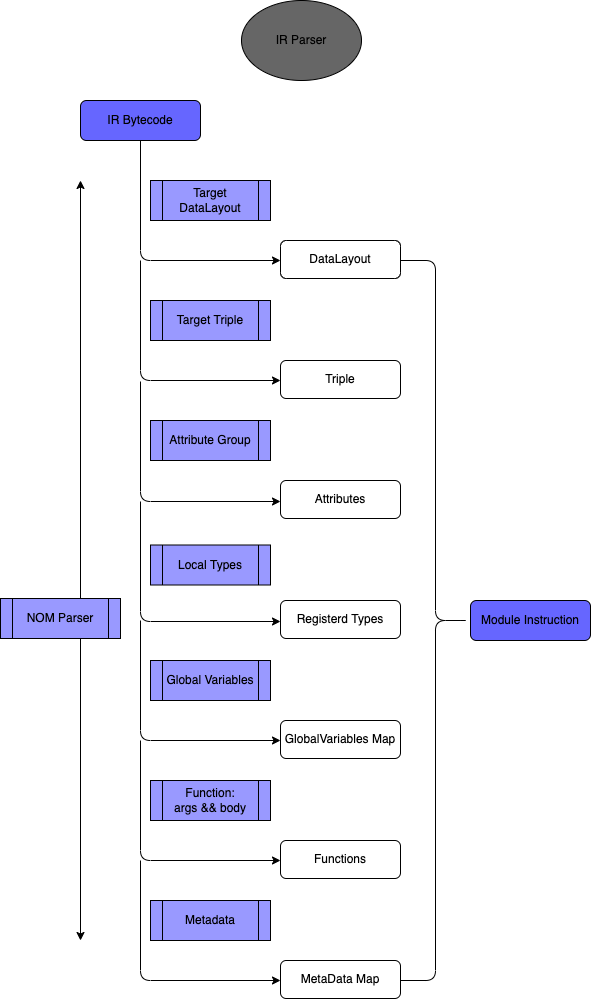
\includegraphics[width=0.6\textwidth]{ola-lang-backend-parser.png}
    \caption{Ola-lang Backend Parser Pipeline}
    \label{fig:ola-lang-backend-parser}
\end{figure}
\end{itemize}
